\section{Observation, Calculation}
	\begin{table}[H]
	\centering
	\resizebox{\columnwidth}{!}{%
		\begin{tabular}{|c|c|c|c|}
			\hline
			\textbf{Sl. No.} & \textbf{$V_{in}$ (V)} & \textbf{Binary Output} & \textbf{Equivalent Voltage} \\ \hline
			1                & 0.1                   & 00000101               & 0.10                        \\
			2                & 0.5                   & 00011001               & 0.49                        \\
			3                & 1.0                   & 00110011               & 1.00                        \\
			4                & 1.5                   & 01001100               & 1.49                        \\
			5                & 2.0                   & 01100110               & 2.00                        \\
			6                & 2.5                   & 01111111               & 2.49                        \\
			7                & 3.0                   & 10011001               & 3.00                        \\
			8                & 3.5                   & 10110010               & 3.49                        \\
			9                & 4.0                   & 11001100               & 4.00                        \\
			10               & 4.5                   & 11100101               & 4.49                        \\
			11               & 5.0                   & 11111111               & 5.00                        \\ \hline
		\end{tabular}%
	}
	\caption{ADC-DAC Observation}
	\label{obs}
\end{table}

	% put the image images/graph.png here with caption and label
	\begin{figure}[h]
		\centering
		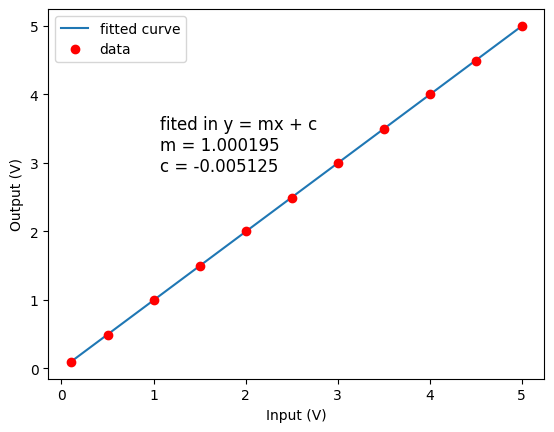
\includegraphics[width=0.8\columnwidth]{images/graph.png}
		\caption{ADC graph}
		\label{graph}
	\end{figure}

	We fit the input and the output using a straight line. Theoretically they should be equal, so the expected slope is 1. From the \hyperref[graph]{Figure 4} we can see that the slope is $1.000195$, with a very minor offset along the y axis of $-0.005125$

	\begin{figure}
		\centering
		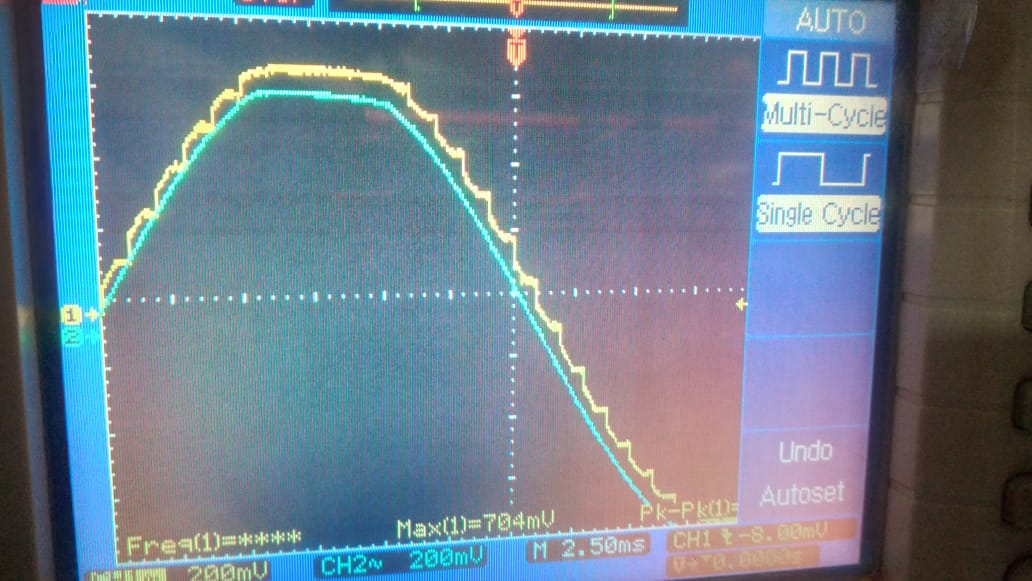
\includegraphics[width=0.8\columnwidth]{images/1.jpg}
		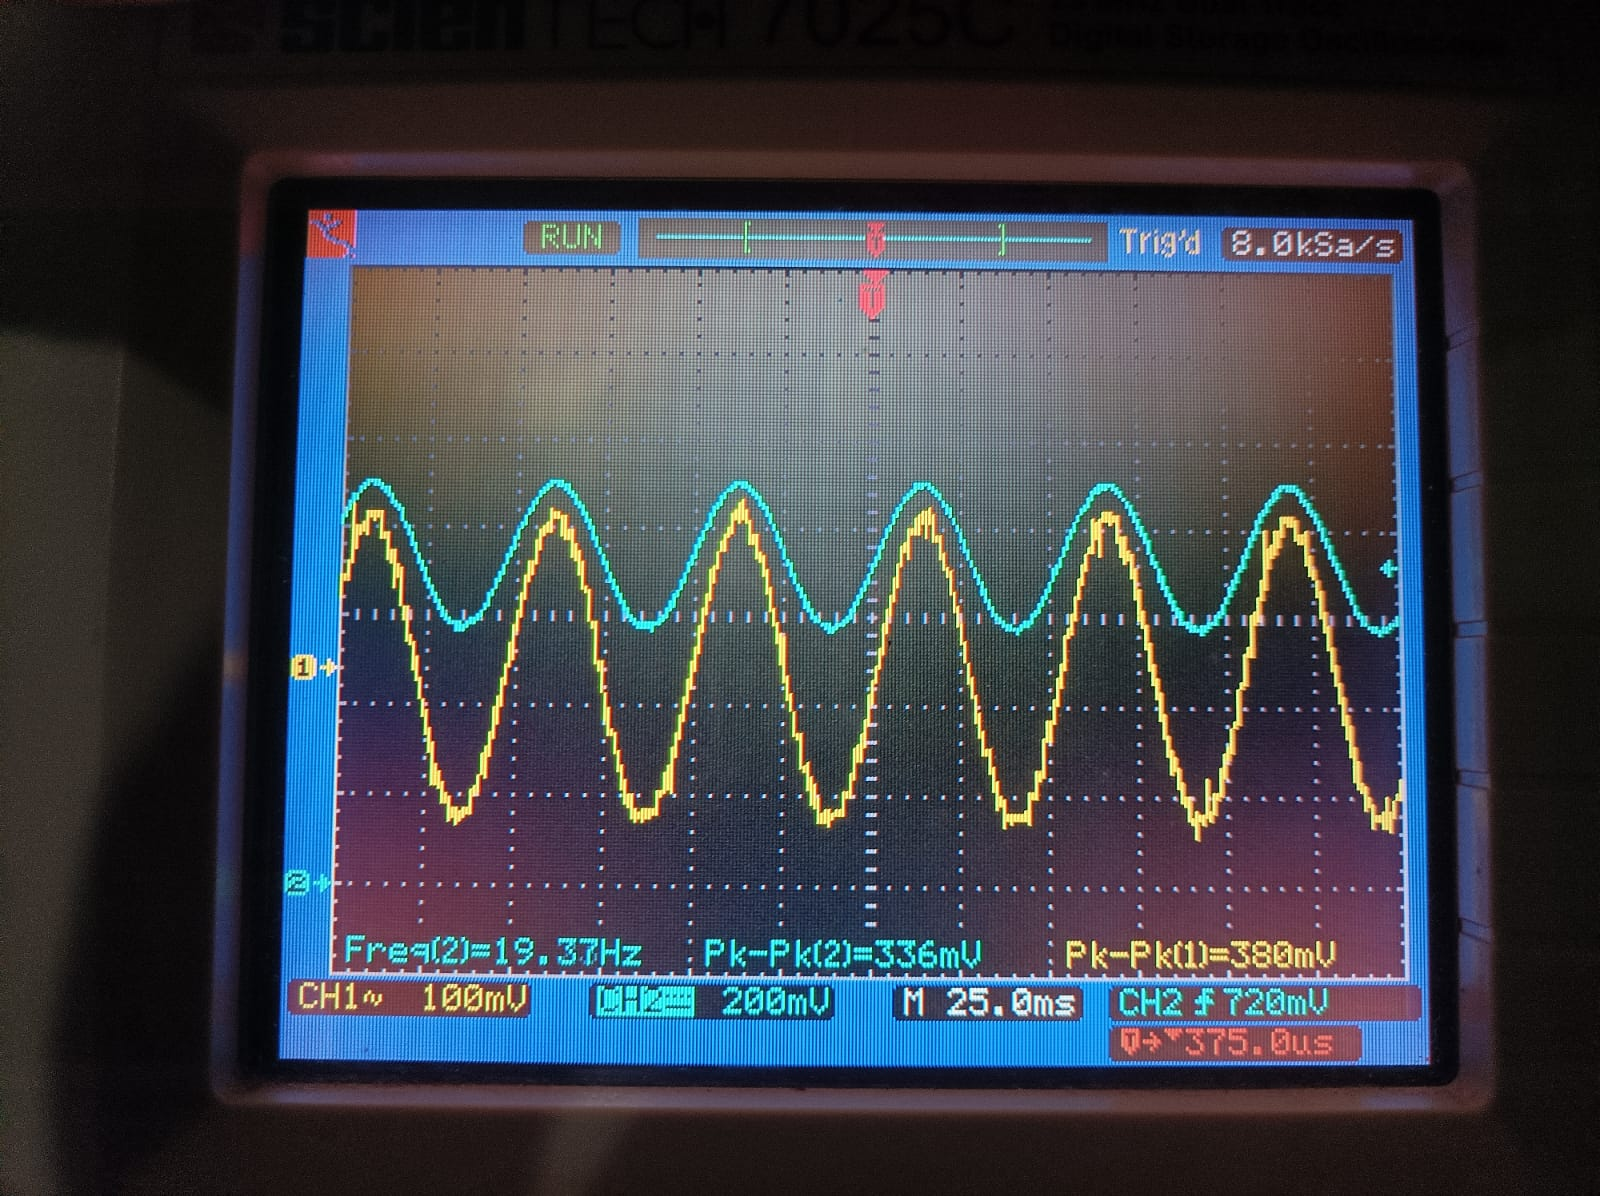
\includegraphics[width=0.8\columnwidth]{images/2.jpg}
		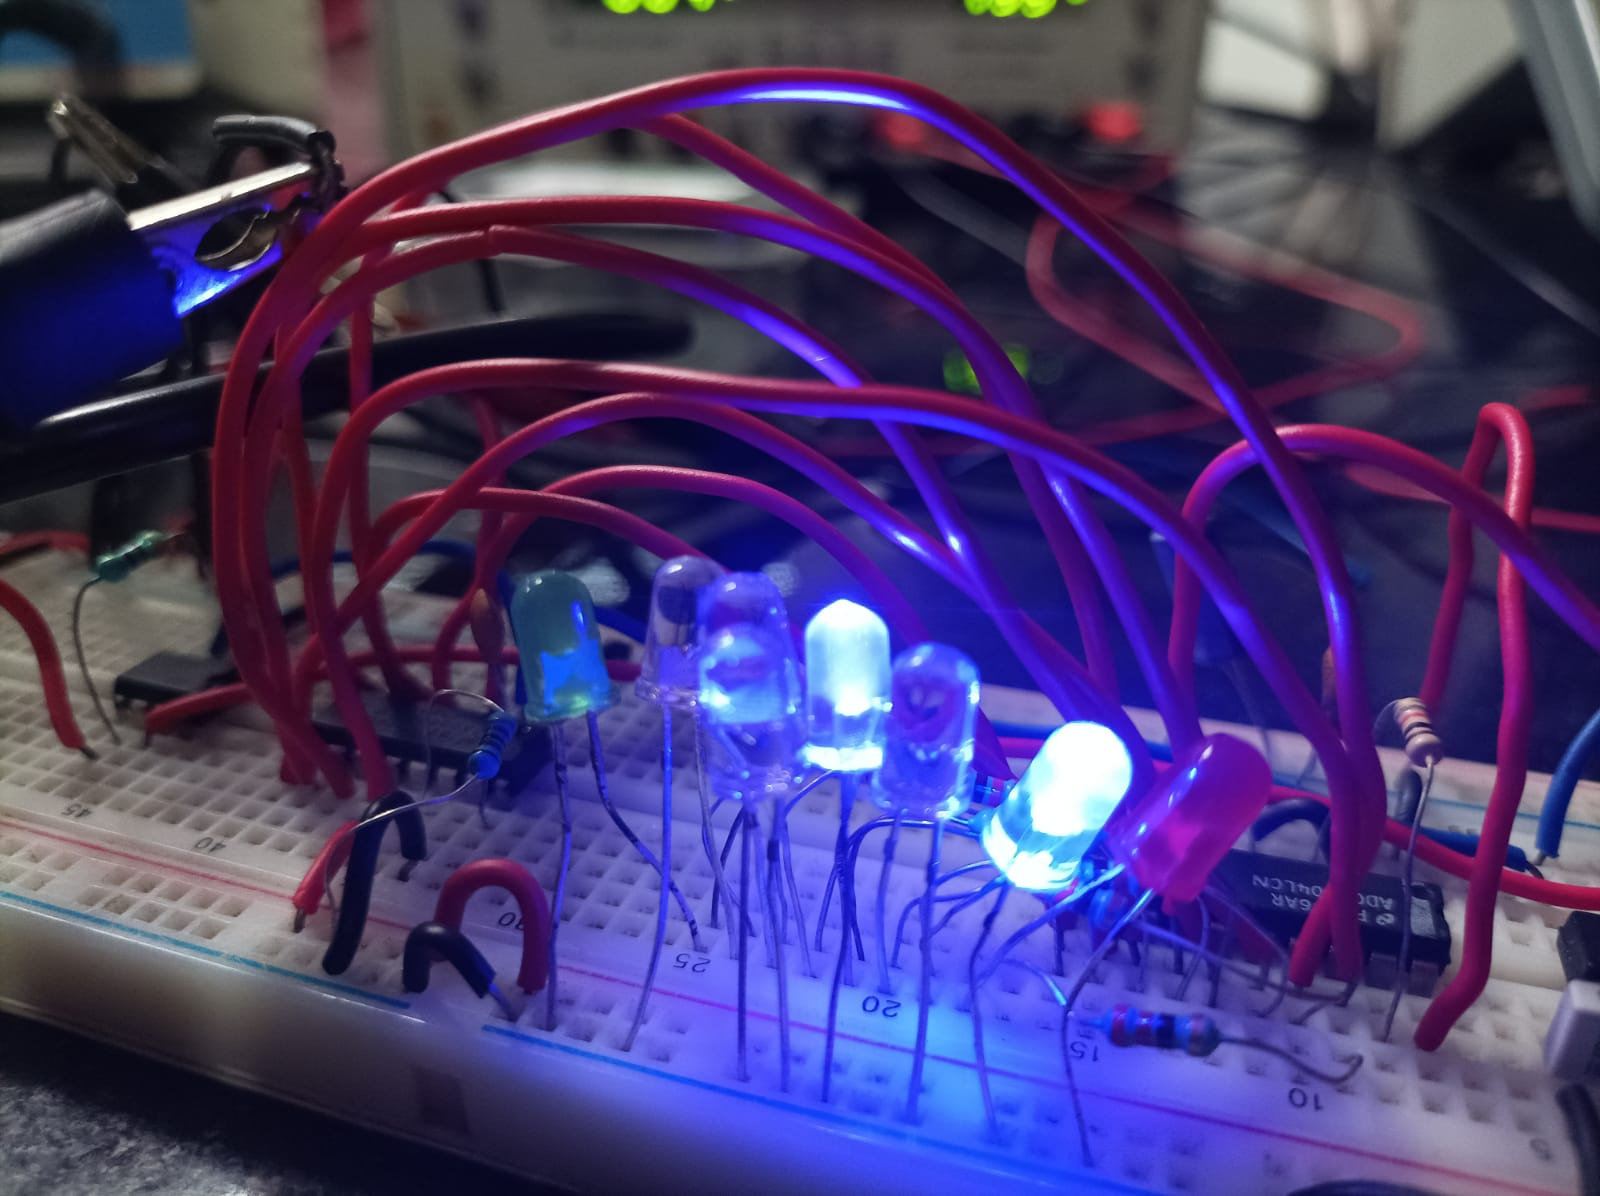
\includegraphics[width=0.8\columnwidth]{images/3.jpg}
	\end{figure}